\labeledsection{First-Order Predicate Logic}{sec:pl1}
\definition{$\text{PL}^1$}{
First-Order (Predicate) Logic $\text{PL}^1$ is a \linkterm{formal system}{formal_system} extensively used in mathematics, philosophy, linguistics, and computer science. It combines \linkterm{$\text{PL}^0$}{def:pl0_as_ls} with the ability to quantify over \linkterm{individuals}{fol_sig}
}{pl1}


\definition{First-Order Signature}{
A First-Order Signature is a tuple $\Sigma := \tuple{\Sigma_1, \linkterm{\Sigma_0}{wff0_def}}$ where $\Sigma_1 := \Sigma^f \cup \Sigma^p \cup \Sigma^{sk}$:
\begin{itemize}
\item $\Sigma^f := \bigcup_{k \in \N} \Sigma_k^f$ of \textbf{function constants} (or \textbf{terms}), where members of $\Sigma_k^f$ denote the $k$-ary \linkterm{functions}{function} on \textbf{individuals}
\item $\Sigma^p := \bigcup_{k \in \N} \Sigma_k^p$ of \textbf{predicate constants}, where member of $\Sigma_k^p$ denote $k$-ary \linkterm{relations}{relation} among individuals
\item $\Sigma^{sk} := \bigcup_{k \in \N} \Sigma_k^{sk}$ of \textbf{Skolem constants} that act as witness constructors
\item All are \linkterm{pairwise disjoint}{pairwise_disjoint}, \linkterm{countable}{countable} \linkterm{sets}{def:set} of symbols for each $k \in \N$.
\end{itemize}
We also assume a \linkterm{set}{def:set} of \textbf{individual variables} $V_{\iota} := \set{X,Y,Z,\cdots}$ which we can quantify over them.
}{fol_sig_pl1}

\commandnote{
\Defref{fol_sig_pl1} is the full FOL Signature. In \linkterm{$\text{PL}^\text{nq}$}{plnq}, we did not explicitly define $\Sigma_0$ (assumed to be there) and we did not need $\Sigma^{sk}$ since no quantification over \linkterm{individuals}{fol_sig} was allowed. That is why in \Defref{fol_sig} we only mentioned what \linkterm{$\text{PL}^\text{nq}$}{plnq} actually uses of the  \linkterm{full FOL Signature}{fol_sig_pl1}
}

\commandnote{
In \linkterm{$\text{PL}^\text{nq}$}{plnq}, we defined terms and formulae in \Defref{wff_terms} and \Defref{wff_formulae_fol} as follows:
\begin{itemize}
    \item We denote the \linkterm{set}{def:set} of all well-formed \linkterm{terms}{fol_sig} over a \linkterm{FOL Signature}{fol_sig} $\Sigma$ with $\text{wff}_{\iota}(\Sigma)$, and the \linkterm{closed}{ground_pl0} ones with $\text{cwff}_{\iota}(\Sigma)$
    \item We denote the \linkterm{set}{def:set} of all well-formed \linkterm{formulae}{fol_sig} over a \linkterm{FOL Signature}{fol_sig} $\Sigma$ with $\text{wff}_o(\Sigma)$, and the \linkterm{closed}{ground_pl0} ones with $\text{cwff}_o(\Sigma)$
\end{itemize}
}

\definition{\linkterm{$\text{PL}^1$}{pl1} Terms}{
The \linkterm{set}{def:set} $\text{wff}_{\iota}(\Sigma_1, V_{\iota})$ of \textbf{well-formed terms} over the signature $\Sigma_1$ and variables \linkterm{$V_{\iota}$}{fol_sig_pl1} is defined by the following \linkterm{grammar}{phrase_structure_grammar}:
\begin{align*}
f^k \quad &\in \quad \Sigma_k^f \cup \Sigma_k^{sk} \\
X \quad &\in \quad \linkterm{V_{\iota}}{fol_sig_pl1} \\ 
t \quad &::= \quad X \mid f^k(t_1, \cdots, t_k)
\end{align*}
}{terms_pl1}


\definition{\linkterm{$\text{PL}^1$}{pl1} Propositions}{
The \linkterm{set}{def:set} $\text{wff}_{\circ}(\Sigma_1, V_{\iota})$ of \textbf{well-formed formulae} over the signature $\Sigma_1$ and variables \linkterm{$V_{\iota}$}{fol_sig_pl1} is defined by the following \linkterm{grammar}{phrase_structure_grammar}:
\begin{align*}
p^k \quad &\in \quad \Sigma_k^p \\
t_i \quad &\in \quad \text{wff}_{\iota}(\Sigma_1, \linkterm{V_{\iota}}{fol_sig_pl1}) \\ 
X \quad &\in \quad \linkterm{V_{\iota}}{fol_sig_pl1} \\ 
A \quad &::= \quad p^k(t_1, \cdots, t_k) \mid \top \mid \neg A \mid A \land A \mid \forall X.A
\end{align*}
}{formulae_pl1}

\definition{Universal Quantifier}{
The \textbf{universal quantifier} $\forall$ is a binding operator used to express $\forall X.A$, i.e. a \linkterm{formula}{formulae_pl1} $A$ holds for all possible values of an \linkterm{individual variable}{terms_pl1} $X \in$ \linkterm{$V_{\iota}$}{fol_sig_pl1}
}{forall}

\commandnote{
Notice that we only need $\top, \land, \neg$ as connectives because the others ($\bot, \lor, \Rightarrow, \Leftrightarrow$) are defined via \textbf{abbreviations}:
\begin{itemize}
    \item $\bot := \neg \top$
    \item $A \lor B := \neg (\neg A \land \neg B)$
    \item $A \Rightarrow B := \neg A \lor B$
    \item $A \Leftrightarrow B := (A \Rightarrow B) \land (B \Rightarrow A)$ 
\end{itemize}
}

\definition{Existential Quantifier}{
The \textbf{existential quantifier} $\exists$ is a binding operator defined as an \textbf{abbreviation} for a negated universal statement: $\exists X.A :\equiv \neg (\forall X. \neg A)$. It allows us to express that at least one \linkterm{individual}{terms_pl1} satisfies the \linkterm{formula}{formulae_pl1} $A$.
}{exists}

\commandnote{
\textbf{Remember:} \Defref{var_occ_pl0} , \Defref{ground_pl0} for \linkterm{$\text{PL}^0$}{def:pl0_as_ls}. We have a similar notion of free variables in \linkterm{$\text{PL}^1$}{pl1} that help us define closed/ground \linkterm{$\text{PL}^1$}{pl1} \linkterm{formulae}{formulae_pl1}.
}



\definition{Free Variables}{
An occurrence of a variable $X$ is \textbf{free} in a \linkterm{formula}{formulae_pl1} $A$ if it is not within the scope of a binder. We define the \linkterm{set}{def:set} of free variables in $A$ ($\text{free}(A)$) recursively as follows:
\begin{itemize}
    \item \textbf{For Terms} ($t \in $ \linkterm{$\text{wff}_{\iota}(\Sigma_1, V_{\iota})$}{terms_pl1})
    \begin{itemize}
        \item $\text{free}(X) = \set{X}$
        \item $\text{free}(f^k(t_1, \cdots, t_k)) := \bigcup_{i=1}^{k} \text{free}(t_i)$
    \end{itemize}
    \item \textbf{For Formulae} ($A \in $ \linkterm{$\text{wff}_{\circ}(\Sigma_1, V_{\iota})$}{formulae_pl1})
    \begin{itemize}
        \item $\text{free}(p^k(t_1, \cdots, t_k)) := \bigcup_{i=1}^{k} \text{free}(t_i)$
        \item $\text{free}(\top) := \emptyset$
        \item $\text{free}(\neg A) := \text{free}(A)$
        \item $\text{free}(A \land B) := \text{free}(A) \cup \text{free}(B)$
        \item $\text{free}(\forall X.A) := \text{free}(A) \setminus \set{X}$
    \end{itemize}
\end{itemize}
}{free_vars_pl1}

\definition{Bound Variables}{
An occurrence of a variable $X$ is \textbf{bound} if it occurs within the scope of a quantifier. We define the \linkterm{set}{def:set} of bound variables $\text{BVar}(A)$ as the \linkterm{set}{def:set} of all variables that are \textit{captured} by a binder:
\begin{itemize}
    \item \textbf{For Terms} ($t \in $ \linkterm{$\text{wff}_{\iota}(\Sigma_1, V_{\iota})$}{terms_pl1})
    \begin{itemize}
        \item $\text{BVar}(t) := \emptyset$ (\textit{variables in terms are always free until a formula provides a binder})
    \end{itemize}
    \item \textbf{For Formulae} ($A \in $ \linkterm{$\text{wff}_{\circ}(\Sigma_1, V_{\iota})$}{formulae_pl1})
    \begin{itemize}
        \item $\text{BVar}(p^k(t_1, \cdots, t_k)) := \emptyset$
        \item $\text{BVar}(\neg A) := \text{BVar}(A)$
        \item $\text{BVar}(A \land B) := \text{BVar}(A) \cup \text{BVar}(B)$
        \item $\text{BVar}(\forall X.A) := \text{BVar}(A) \cup \set{X}$
    \end{itemize}
\end{itemize}
}{bound_vars_pl1}

\definition{Ground Formulae}{
A \linkterm{$\text{PL}^1$}{pl1} formula $A$ is called \textbf{ground/closed} iff \linkterm{free}{free_vars_pl1}$(A) := \emptyset$. A closed \linkterm{formula}{formulae_pl1} is called a sentence. We denote the \linkterm{set}{def:set} of all \textbf{ground} \linkterm{terms}{terms_pl1} with $\text{cwff}_{\iota}(\Sigma_1, V_{\iota})$ and the \linkterm{set}{def:set} of all sentences with $\text{cwff}_{\circ}(\Sigma_1, V_{\iota})$
}{ground_pl1}

\definition{Alphabetical Variants}{
\linkterm{Bound variables}{bound_vars_pl1} can be \textbf{renamed}; specifically, if $\forall X.B$ is a sub-formula of $A$, let $A'$ be the result of replacing $\forall X.B$ in $A$ with $\forall Y.B'$, where $B'$ is obtained from $B$ by replacing all occurrences of $X \in \text{free}(B)$ with a new variable $Y$ that does not occur in $A$. We call $A'$ an \textbf{alphabetical variant} of $A$ (and vice versa).
}{alphabetical_variants}


\definition{\linkterm{$\text{PL}^1$}{pl1} Universe}{
\linkterm{$\text{PL}^1$}{pl1} uses the universe $\mathcal{D}_{\text{PL}^1} := \mathcal{D}_0 \cup \mathcal{D}_{\iota}$ where $\mathcal{D}_0 = \set{T,F}$ is the \linkterm{set}{def:set} of truth values and $\mathcal{D}_{\iota} \neq \emptyset$ is a non-empty \linkterm{set}{def:set} of \linkterm{individuals}{fol_sig}
}{domain_pl1}

\definition{Interpretation in \linkterm{$\text{PL}^1$}{pl1}}{
The interpretation function in \linkterm{$\text{PL}^1$}{pl1} \linkterm{assigns}{var_ass_pl0} values to \linkterm{constants}{fol_sig}:
\begin{enumerate}
    \item We use the \linkterm{interpretation}{model_pl0} from \linkterm{$\text{PL}^0$}{def:pl0_as_ls}
        \begin{itemize}
        \item $\func{\mathcal{I}(\neg)}{\mathcal{D}_0}{\mathcal{D}_0}$; $T \mapsto F, F \mapsto T$
        \item $\func{\mathcal{I}(\land)}{\cartprod{\mathcal{D}_0,\mathcal{D}_0}}{\mathcal{D}_0}$; $\tuple{\alpha, \beta} \mapsto T$, iff $\alpha = \beta = T$
        \item $\mathcal{I}(\top) = T$
        \item $\mathcal{I}(\bot) = F$
        \end{itemize}
    \item We interpret \linkterm{individual constants}{fol_sig} as \linkterm{individuals}{fol_sig}:
    $
    \func{\mathcal{I}}{\Sigma_0^f}{\mathcal{D}_{\iota}}
    $
    \item We interpret \linkterm{function constants}{fol_sig} as \linkterm{functions}{function}:
    $
    \mathcal{I}: \Sigma_{k \neq 0}^f \to \mathcal{D}_{\iota}^{k \neq 0} \to \mathcal{D}_{\iota}
    $
    \item We interpret \linkterm{predicate constants}{fol_sig} as \linkterm{relations}{relation}:
    $
    \func{\mathcal{I}}{\Sigma_k^p}{\powerset{\mathcal{D}_{\iota}^{k}}}
    $
\end{enumerate}
}{interpretation_pl1}

\definition{\linkterm{$\text{PL}^1$}{pl1} Value Function}{
Given a model $\tuple{\mathcal{D}, \mathcal{I}}$, the value function $\mathcal{I}_{\varphi}$ is recursively defined:
\begin{enumerate}
\item $\func{\mathcal{I}_{\varphi}}{\linkterm{\text{wff}_{\iota}(\Sigma_1, V_{\iota})}{terms_pl1}}{\mathcal{D}_{\iota}}$ assigns values to \linkterm{terms}{terms_pl1} 
\begin{itemize}
    \item $\mathcal{I}_{\varphi}(X) := \varphi(X)$, and
    \item $\mathcal{I}_{\varphi}(f(A_1, \cdots, A_k)) := \mathcal{I}(f)(\mathcal{I}_{\varphi}(A_1), \cdots, \mathcal{I}_{\varphi}(A_k))$
\end{itemize}
\item $\func{\mathcal{I}_{\varphi}}{\linkterm{\text{wff}_{\circ}(\Sigma_1, V_{\iota})}{formulae_pl1}}{\mathcal{D}_{\circ}}$ assigns values to \linkterm{formulae}{formulae_pl1}
\begin{itemize}
    \item $\mathcal{I}_{\varphi}(\top) = \mathcal{I}(\top) = T$
    \item $\mathcal{I}_{\varphi}(\neg A) := \mathcal{I}(\neg) (\mathcal{I}_{\varphi}(A))$
    \item $\mathcal{I}_{\varphi} (A \land B) := \mathcal{I}(\land) (\mathcal{I}_{\varphi}(A), \mathcal{I}_{\varphi}(B))$
    \item $\mathcal{I}_{\varphi}(p(A_1, \cdots, A_k)) := T, \text{ iff } \tuple{\mathcal{I}_{\varphi}(A_1), \cdots, \mathcal{I}_{\varphi}(A_k)} \in \mathcal{I}(p)$ 
    \item $\mathcal{I}_{\varphi}(\forall X.A) := T, \text{ iff } \mathcal{I}_{\varphi, [a/X]}(A) = T \text{ for all } a \in \mathcal{D}_{\iota}$
\end{itemize}
\end{enumerate}
}{value_function_pl1}


\definition{Assignment Extension}{
Let $\varphi: V_{\iota} \to \mathcal{D}_{\iota}$ be a \textbf{variable assignment} and $a \in \mathcal{D}_{\iota}$. The \textbf{extension} of $\varphi$ by $a$ for $X$, denoted by $\varphi,[a/X]$ is a variable assignment defined as:
\[
\varphi,[a/X](Y) := \begin{cases} 
a & \text{if } Y = X \\ 
\varphi(Y) & \text{if } Y \neq X 
\end{cases}
\]
Equivalently, viewing the assignment as a set of ordered pairs:
\[
\varphi,[a/X] = \{(Y, \varphi(Y)) \mid Y \in V_{\iota} \setminus \{X\}\} \cup \{(X, a)\}
\]
This assignment coincides with $\varphi$ for all variables except $X$, where it maps to the individual $a$.
}{assignment_extension_pl1}

\definition{Expression Language}{
Let signature $\Sigma$ and variables $\mathcal{V}$ be \linkterm{disjoint sets}{disjoint} and $G$ a \linkterm{grammar}{phrase_structure_grammar} whose vocabulary is $\Sigma \cup \mathcal{V}$, then we call $\tuple{\Sigma, \mathcal{V}, G}$ an \textbf{expression language}, and denote the \linkterm{language}{formal_language} of $G$ with $\text{wfe}(\Sigma, \mathcal{V})$: the \linkterm{set}{def:set} of \textbf{well-formed expressions}.
}{expression_language}

\commandnote{
For \linkterm{$\text{PL}^1$}{pl1}, we have:
\[
\text{wfe}(\Sigma_1, \mathcal{V}_{\iota}) := \text{wff}_{\circ}(\Sigma_1, V_{\iota}) \cup \text{wff}_{\iota}(\Sigma_1, V_{\iota})
\]
}

\definition{Support}{
Let $f: A \to B$ be a \linkterm{function}{function}. The \textbf{support} of $f$, denoted by $\text{supp}(f)$, is the \linkterm{set}{def:set} of all elements in the \linkterm{domain}{domain_codomain} $A$ for which the \linkterm{function}{function} does not return a "default" or "identity" value. 
}{support_function}

\definition{Substitution}{
Let \linkterm{$\text{wfe}(\Sigma, \mathcal{V})$}{expression_language} be an \linkterm{expression language}{expression_language}, then we call $\func{\sigma}{\mathcal{V}}{\text{wfe}(\Sigma, \mathcal{V})}$ a \textbf{substitution} iff the \linkterm{support}{support_function} $\text{supp}(\sigma) := \set{X \mid (X,A) \in \sigma \land X \neq A}$ of $\sigma$ is \linkterm{finite}{set_cardinality}. We denote the \textbf{empty substitution} with $\epsilon$.
}{substitution}

\definition{}{
We can \textbf{discharge} a variable $X$ from a \linkterm{substitution}{substitution} $\sigma$ by setting $\sigma_{-X} := \sigma , [X/X]$
}{discharge_substitution}

\definition{}{
Let $\sigma$ be a \linkterm{substitution}{substitution}, then we call $\text{intro}(\sigma) := \bigcup_{X \in \text{supp}(\sigma)} \text{free}(\sigma(X))$ the \linkterm{set}{def:set} of variables \textbf{introduced} by $\sigma$.
}{substitution_introduced}

\textbf{Example: }consider the \linkterm{formula}{formulae_pl1} $A := \forall X. p(X,Y)$ and the \linkterm{substitution}{substitution} $\sigma := \set{[Z / Y]}$:
\begin{itemize}
    \item $\text{supp}(\sigma) = \set{Y}$
    \item $\text{free}(\sigma(Y)) = \text{free}(Z) = \set{Z}$
    \item $\text{intro}(\sigma) = \text{free}(\sigma(Y)) = \set{Z}$
\end{itemize}

\definition{Substitution Application}{
We define substitution application by:
\begin{itemize}
    \item $\sigma(c) = c$ for $c \in \Sigma$
    \item $\sigma(X) = A$ iff $X \in \mathcal{V}$ and $(X,A) \in \sigma$
    \item $\sigma(f(A_1, \cdots, A_n)) = f(\sigma(A_1), \cdots, \sigma(A_n))$
    \item $\sigma(\forall X.A) = \forall X.\sigma_{-X}(A)$
\end{itemize}
}{substitution_application}

\commandnote{
The concept of \linkterm{support}{support_function} is useful to handle \linkterm{finiteness}{set_cardinality} in systems that are \linkterm{infinite}{set_cardinality}. For example, in \linkterm{$\text{PL}^1$}{pl1}, the \linkterm{set}{def:set} of variables $\mathcal{V}_{\iota}$ is \linkterm{infinite}{set_cardinality}. However, when we \linkterm{apply a substitution}{substitution_application}, we don't want to deal with an \linkterm{infinite}{set_cardinality} number of changes. By requiring the \linkterm{support}{support_function} of a \linkterm{substitution}{substitution} to be \linkterm{finite}{set_cardinality}, we ensure that only a managable, \linkterm{countable}{countable} number of variables are being modified, while the \linkterm{infinite}{set_cardinality} rest of them simply stay the same (mapping to their \textit{"identity"} value).
}

\textbf{Substitution Example}: consider the formula $g(x,y, h(z))$, and we want to \linkterm{apply}{substitution_application} the \linkterm{substitution}{substitution} $\sigma := \set{x \mapsto a, y \mapsto f(b), z \mapsto a}$ we get the formula $g(a, f(b), h(a))$

\commandnote{
Usually we use another notation for writing the \linkterm{substitution}{substitution} $\sigma := \set{x \mapsto a, y \mapsto f(b), z \mapsto a}$ which is $[a/x], [f(b) / y], [a / z]$ where $[A / X]$ (read as \textit{A for X} i.e. substitute $X$ with $A$) $\equiv X \mapsto A \equiv (X,A) \in \sigma$  
}

\definition{Substitution Extension}{
Let $\sigma$ be a \linkterm{substitution}{substitution}, then we denote the \textbf{extension} of $\sigma$ with $[A / X]$ by $\sigma , [A / X]$ and define it as $\set{(Y,B) \in \sigma \mid Y \neq X} \cup \set{(X,A)}$.
}{substitution_extension}

\definition{Capture-Avoiding Substitution Application}{
Let $\sigma$ be a \linkterm{substitution}{substitution}, $A$ a \linkterm{formula}{formulae_pl1}, and $A'$ an \linkterm{alphabetical variant}{alphabetical_variants} of $A$, such that $\text{intro}(\sigma) \cap \text{BVar}(A') = \emptyset$. Then we define \textbf{capture-avoiding substitution application} via $\sigma(A) := \sigma(A')$
}{subst_app_avoid_capture}

\commandnote{
We said $\sigma(\forall X.A) = \forall X.\sigma_{-X}(A)$ but this can lead to \refterm{variable capture}{variable_capture}, i.e. $[f(X) / Y](\forall X.p(X,Y))$ would evaluate to $\forall X.p(X,f(X))$ where the second occurrence of $X$ is now \linkterm{bound}{bound_vars_pl1} whereas it was \linkterm{free}{free_vars_pl1} before.

The solution for this is to \linkterm{rename}{alphabetical_variants} the \linkterm{bound variable}{bound_vars_pl1} $X$ in $\forall X.p(X,Y)$ before \linkterm{applying}{substitution_application} the \linkterm{substitution}{substitution} and there where we need \linkterm{capture-avoiding substitution application}{subst_app_avoid_capture} 
}

\textbf{Example:} we want to \linkterm{apply}{substitution_application} $\sigma := \set{[f(X) / Y]}$ to the \linkterm{formula}{formulae_pl1} $A = \forall X. p(X,Y)$
\begin{itemize}
    \item $\text{intro}(\sigma) \cap \text{BVar}(A) = \set{X} \cap \set{X} = \set{X}$ 
    \item Hence, we need to find an \linkterm{alphabetical variant}{alphabetical_variants} $A'$ for $A$, say $A' = \forall Z. p(Z,Y)$
    \item Now $\text{intro}(\sigma) \cap \text{BVar}(A') = \set{X} \cap \set{Z} = \emptyset$
    \item Hence, we define $\sigma(A) = \sigma(A')$
    \item $\sigma(A') = \sigma(\forall Z. p(Z,Y)) = \forall Z. \sigma_{-Z} (p(Z,Y))$
    \item $[f(X) / Y](p(Z,Y)) = p(Z,f(X))$
    \item $\sigma(A) = \sigma(A') = \forall Z.p(Z,f(X))$
\end{itemize}

\Lemma{
Let $A$ and $B$ be \linkterm{terms}{terms_pl1}, then $\mathcal{I}_{\varphi}([B / X](A)) = \mathcal{I}_{\psi}(A)$, where $\psi = \varphi , [\mathcal{I}_{\varphi}(B) / X]$.    
}{lem_subs_terms}
\Proof{
By induction on the depth of $A$:
\begin{enumerate}
\item $\text{depth} = 0$

Then $A$ is either a variable or a constant. If $A$ is variable, say $Y$, we have two cases $Y=X$ and $Y \neq X$:
\begin{enumerate}
    \item $A = Y = X$: 
    
    then $\mathcal{I}_{\varphi}([B / X](A)) = \mathcal{I}_{\varphi}([B / X](X)) = \mathcal{I}_{\varphi}(B) = \psi(X) = \mathcal{I}_{\psi}(X) = \mathcal{I}_{\psi}(A)$

    \item $A = Y \neq X$:
    
    then $\mathcal{I}_{\varphi}([B / X](A)) = \mathcal{I}_{\varphi}([B / X](Y)) = \mathcal{I}_{\varphi}(Y) = \varphi(Y) = \psi(Y) = \mathcal{I}_{\psi}(Y) = \mathcal{I}_{\psi}(A)$

    \item $A$ is a constant $\leadsto$ analogous to 1.b
\end{enumerate}  
\item $\text{depth} > 0$

then $A = f(A_1, \cdots, A_n)$ and we have
\begin{align*}
\mathcal{I}_{\varphi}([B / X](A)) \quad &= \quad \mathcal{I}(f) (\mathcal{I}_{\varphi}([B / X](A_1)), \cdots, \mathcal{I}_{\varphi}([B / X](A_n))) \\
 \quad &= \quad \mathcal{I}(f)(\mathcal{I}_{\psi}(A_1), \cdots, \mathcal{I}_{\psi}(A_n)) \\
 \quad &= \quad \mathcal{I}_{\psi}(A)
\end{align*}
by induction hypothesis
\end{enumerate}
}

\Lemma{
Let $A$ and $B$ be \linkterm{propositions}{formulae_pl1}, then $\mathcal{I}_{\varphi}([B / X]A) = \mathcal{I}_{\psi}(A)$, where $\psi = \varphi , [\mathcal{I}_{\varphi}(B) / X]$.    
}{lem_subs_formulae}

\Proof{
By induction on the number of $n$ connectives and quantifiers in $A$:
\begin{enumerate}
\item $n=0$

then $A$ is an \linkterm{atomic formula}{atomic_formula}, and we can argue like in the induction step of the \Lemref{lem_subs_terms}
\item $n>0$ and $A = \neg B$ or $A = C \circ D$

Here we argue like in the induction step of \Lemref{lem_subs_terms} as well
\item $n>0$ and $A = \forall Y.C$ where (\linkterm{WLOG}{def:wlog}) $X \neq Y$ (otherwise, \linkterm{rename}{alphabetical_variants})
\begin{enumerate}
\item then $\mathcal{I}_{\psi}(A) = \mathcal{I}_{\psi}(\forall Y.C) = T$, iff $\mathcal{I}_{\psi, [a / Y]}(C) = T$ for all $a \in \mathcal{D}_{\iota}$
\item But $\mathcal{I}_{\psi, [a / Y]}(C) = \mathcal{I}_{\varphi, [a / Y]}([B / X](C)) = T$, by induction hypothesis.
\item So $\mathcal{I}_{\psi}(A) = \mathcal{I}_{\varphi}(\forall Y.[B / X](C)) = \mathcal{I}_{\varphi}([B / X](\forall Y.C)) = \mathcal{I}_{\varphi}([B / X](A))$ 
\end{enumerate}
\end{enumerate}
}

\definition{$\mathcal{ND}_1$}{
\textbf{The First-Order Natural Deduction Calculus} extends \linkterm{$\mathcal{ND}_0$}{nd_0} by the following four \linkterm{inference rule}{inference_rules_logic}:
\begin{tcolorbox}[colback=white, colframe=black, sharp corners, boxrule=0.5pt]
    \begin{multicols}{2}
        % impl. intro
        \noindent
        \begin{minipage}{\linewidth}
            \[
                \infer[\forall I^{*}]{\forall X. A}{A}
            \]
        \end{minipage}
    
        % impl. elim.
        \noindent
        \begin{minipage}{\linewidth}
            \[
                \infer[\forall E]{[B/X](A)}{\forall X.A}
            \]
        \end{minipage}
    \end{multicols}
    
    * means that $A$ does not depend on any hypothesis in which $X$ is \linkterm{free}{free_vars_pl1}

    \begin{multicols}{2}
        \noindent
        \begin{minipage}{\linewidth}
            \vspace{0.8cm}
            \[
                \infer[\exists I]{\exists X.A}{[B/X](A)}
            \]
        \end{minipage}
    
        \noindent
        \begin{minipage}{\linewidth}
            \[
                \infer[\exists E^1]{C}{
                    \exists X.A \qquad
                    \infer*{C}{[[c/X](A)]^1} \qquad
                    c \in \sum_{0}^{sk} \text{new} \qquad
                }                    
            \]
        \end{minipage}
    \end{multicols}
\end{tcolorbox}
}{nd1}


\commandnote{
If our knowledge base has $\text{loves}(\text{Anna}, \text{Anna})$, using $\exists I$ we can infer several things, e.g.:
\begin{itemize}
    \item $\exists X. \text{loves}(X,X)$
    \item $\exists X. \text{loves}(X, \text{Anna})$
    \item $\exists X. \text{loves}(\text{Anna},X)$
    \item $\exists X \exists Y. \text{loves}(X,Y)$
\end{itemize}
Hence, you might see the rule written in the following notation:
\[
    \infer[\exists I]{\exists X.A(\cdots c \cdots X \cdots)}{A(\cdots c \cdots c \cdots)}
\]
to emphasize that we do not need to \linkterm{replace}{replacement} all instances of the \linkterm{terms}{terms_pl1} $c$ with the variable $X$ (but we can!)
}

\minititle{Notes on $\forall I$}
If we are trying to introduce something of the form $\forall X.A$, conceptually, this is a tricky thing to do! Because how could we prove that $A$ holds for everything! It is not practical to go through every \linkterm{individuals}{terms_pl1}! Therefore, we need a clever way of doing that. 

Let's compare between two types of reasoning that involve generalization, first, let's see the following one:

\begin{figure}[H]
    \centering
    \begin{tcolorbox}[colback=white, colframe=black, sharp corners, boxrule=0.5pt]
        \renewcommand{\arraystretch}{1.3} 
        \begin{tabular}{r l l}
            \textbf{Step} & \textbf{Formula} & \textbf{Rule Applied} \\
            \hline
            (1) & $\text{Blonde}(\text{Anna})$ & Assumption \\
            (2) & $\text{Blonde}(\text{Anna}) \lor \text{Brown}(\text{Anna})$ & $\lor I_l$ (on 1) \\
            (3) & $\text{Blonde}(\text{Anna}) \Rightarrow (\text{Blonde}(\text{Anna}) \lor \text{Brown}(\text{Anna}))$ & $\Rightarrow I^1$ (on 1, 2) $\leadsto$ Discharge (1) \\
            (4) & $\forall X. (\text{Blonde}(X) \Rightarrow (\text{Blonde}(X) \lor \text{Brown}(X)))$ & $\forall I$ (on 3) \\
        \end{tabular}
    \end{tcolorbox}
\end{figure}


That was a \textbf{valid} reasoning. Now let's see another one that looks \textit{(similar)}:
\begin{figure}[H]
    \centering
    \begin{tcolorbox}[colback=white, colframe=black, sharp corners, boxrule=0.5pt]
        \renewcommand{\arraystretch}{1.3} 
        \begin{tabular}{r l l}
            \textbf{Step} & \textbf{Formula} & \textbf{Rule Applied} \\
            \hline
            (1) & $\text{Blonde}(\text{Anna})$ & Assumption \\
            (2) & $\text{Tall}(\text{Anna})$ & Assumption \\
            (3) & $\text{Blonde}(\text{Anna}) \land \text{Tall}(\text{Anna})$ & $\land I$ (on 1,2) \\
            (4) & $\text{Tall}(\text{Anna}) \Rightarrow (\text{Blonde}(\text{Anna}) \land \text{Tall}(\text{Anna}))$ & $\Rightarrow I^2$ (on 2,3) $\leadsto$ Discharge (2) \\
            (5) & $\forall X. (\text{Tall}(X) \Rightarrow (\text{Blonde}(X) \land \text{Tall}(X)))$ & $\forall I$ (on 4) \\
        \end{tabular}
    \end{tcolorbox}
\end{figure}

That was \text{invalid} reasoning in an obvious way! Just because someone is tall, that doesn't mean they are both tall and blonde!

The difference is in the way the \linkterm{individuals}{terms_pl1} "Anna" was used. In the incorrect proof, we assumed Anna is blonde, then we assumed something further about her (being tall), under that new assumption we inferred she's both tall and blonde and then we inferred something further to conclude everyone is like that!

In the correct one, however, we derived the formula from one assumption about Anna and Anna did not appear anywhere before that. Anna was just an \textit{arbitrary} name.

Therefore, the rule might also be written in a different notation:
\[
    \infer[\forall I]{\forall X. A(\cdots X \cdots X \cdots)}{A(\cdots c \cdots c \cdots)}
\]

where $c$ is arbitrary and $X \notin A$ 


\definition{$\mathcal{ND}^1_{\vdash}$}{
The \linkterm{inference rules}{inference_rules_logic} of the \textbf{First-Order Sequent Style Natural Deduction Calculus} consist of those from \linkterm{$\mathcal{ND}^{0}_{\vdash}$}{nd0_seq} plus the following quantifiers rules:
\begin{tcolorbox}[colback=white, colframe=black, sharp corners, boxrule=0.5pt]
    \begin{multicols}{2}
        % impl. intro
        \noindent
        \begin{minipage}{\linewidth}
            \[
                \infer[\forall I]{\Gamma \vdash \forall X. A}{\Gamma \vdash A \quad X \notin \text{free}(\Gamma)}
            \]
        \end{minipage}
    
        % impl. elim.
        \noindent
        \begin{minipage}{\linewidth}
            \[
                \infer[\forall E]{\Gamma \vdash [B/X](A)}{\Gamma \vdash \forall X.A}
            \]
        \end{minipage}
    \end{multicols}
    
    \begin{multicols}{2}
        \noindent
        \begin{minipage}{\linewidth}
            \[
                \infer[\exists I]{\Gamma \vdash \exists X.A}{\Gamma \vdash [B/X](A)}
            \]
        \end{minipage}
    
        \noindent
        \begin{minipage}{\linewidth}
            \[
                \infer[\exists E^1]{\Gamma \vdash C}{
                    \Gamma \vdash \exists X.A \quad 
                    \Gamma , [c/X]A \vdash C \quad
                    c \in \Sigma_0^{\text{sk}} \text{new}
                }                    
            \]
        \end{minipage}
    \end{multicols}
\end{tcolorbox}
}{nd1_seq}

\newpage
\definition{$\text{PL}^1_{=}$}{
We extend \linkterm{$\text{PL}^1$}{pl1} with a new logical constant for \textbf{equality} $= \in \Sigma^p_2$ and fix its \linkterm{interpretation}{interpretation_pl1} to $\mathcal{I}(=) := \set{(x,x) \mid x \in \mathcal{D}_{\iota}}$. We call the extended logic \textbf{First-Order Logic with Equality}.
}{pl1=}

\definition{Position}{
A position is a finite sequence of natural numbers $p = \langle i_1, i_2, \dots, i_n \rangle$ that describes a path from the root of a \linkterm{well-formed expression}{expression_language} to a specific sub-node.
For an \linkterm{expression}{expression_language} $A$, the subexpression at position $p$ is denoted by $A|_p$.
We write $C[A]_p$ to indicate that the expression $C$ contains the subexpression $A$ at position $p$.
If $A$ is an \linkterm{atomic formula}{atomic_formula}, we call $p$ an \textbf{occurrence} of $A$ in $C$.
}{position}

\commandnote{
\begin{minipage}{0.5\textwidth}
\textbf{Example: }consider $C := (p \land q) \Rightarrow r$
\begin{itemize}
    \item \linkterm{Position}{position} $\tuple{1}$ is the subexpression $(p \land q)$
    \item \linkterm{Position}{position} $\tuple{1,1}$ is the \linkterm{occurrence}{position} of the \linkterm{atom}{atomic_formula} $p$
    \item \linkterm{Position}{position} $\tuple{2}$ is the \linkterm{occurrence}{position} of the \linkterm{atom}{atomic_formula} $r$
\end{itemize}
\end{minipage}
\begin{minipage}{0.5\textwidth}
\centering
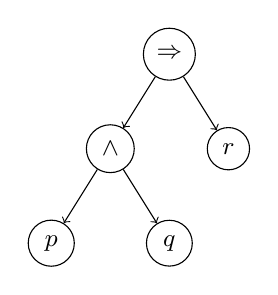
\begin{tikzpicture}[
  level distance=1.2cm,
  sibling distance=1.5cm,
  edge from parent/.style={draw, ->},
  every node/.style={circle, draw, minimum size=3mm, font=\small}
]

\node {$\Rightarrow$}
  child {
    node {$\land$} 
    child { node {$p$} } 
    child { node {$q$} } 
  }
  child {
    node {$r$} 
  };

\end{tikzpicture}
\end{minipage}
}

\definition{Replacement}{
Let $p$ be a \linkterm{position}{position}, then $[A / p]C$ is the \linkterm{expression}{expression_language} obtained from $C$ by \textbf{replacing} the subexpression at $p$ by $A$
}{replacement}

\definition{$\mathcal{ND}^1_{=}$}{
\textbf{The First-Order Logic with Equality Natural Deduction Calculus} extends \linkterm{$\mathcal{ND}_1$}{nd1} by the following two \linkterm{inference rule}{inference_rules_logic}:
\begin{tcolorbox}[colback=white, colframe=black, sharp corners, boxrule=0.5pt]
    \begin{multicols}{2}
        \noindent
        \begin{minipage}{\linewidth}
            \[
                \infer[{=I}]{A = A}{}
            \]
        \end{minipage}
    
        \noindent
        \begin{minipage}{\linewidth}
            \[
                \infer[{=E}]{[B/p] C}{A = B \quad C[A]_p}
            \]
        \end{minipage}
    \end{multicols}
\end{tcolorbox}
}{nd1=}

\commandnote{
\linkterm{equivalence}{equivalent_formulae} ($\Leftrightarrow$) behaves exactly as equality ($=$) 
}

\definition{}{
$\Leftrightarrow I$ is \linkterm{derivable}{derived_inference_rule} and $\Leftrightarrow E$ is \linkterm{admissible}{admissible_inference_rule} in \linkterm{$\mathcal{ND}_1$}{nd1}:
\begin{tcolorbox}[colback=white, colframe=black, sharp corners, boxrule=0.5pt]
    \begin{multicols}{2}
        \noindent
        \begin{minipage}{\linewidth}
            \[
                \infer[{\Leftrightarrow I}]{A \Leftrightarrow A}{}
            \]
        \end{minipage}
    
        \noindent
        \begin{minipage}{\linewidth}
            \[
                \infer[{\Leftrightarrow E}]{[B/p] C}{A \Leftrightarrow B \quad C[A]_p}
            \]
        \end{minipage}
    \end{multicols}
\end{tcolorbox}
}{equiv_rules}


\Figref{fig:nd_rules_all} shows all \linkterm{inference rules}{inference_rules_logic} of the natural deduction calculus, i.e. the \linkterm{union}{set_union} of \linkterm{$\mathcal{ND}_0$}{nd_0}, \linkterm{$\mathcal{ND}_1$}{nd1}, \linkterm{$\mathcal{ND}^1_{=}$}{nd1=}, and \linkterm{equivalence rules}{equiv_rules}

\begin{figure}[H]
    \centering
    \begin{tcolorbox}[colback=white, colframe=black, sharp corners, boxrule=0.5pt]
        
        \begin{multicols}{3}
            % conj. intro
            \noindent
            \begin{minipage}{\linewidth}   
                \[
                    \infer[\land I]{A \land B}{A & B}
                \]
            \end{minipage}
        
            % conj. elimL
            \noindent
            \begin{minipage}{\linewidth}   
                \[
                    \infer[\land E_l]{A}{A \land B}
                \]
            \end{minipage}
        
            % conj. elimR
            \noindent
            \begin{minipage}{\linewidth}   
                \[
                    \infer[\land E_r]{B}{A \land B}
                \]
            \end{minipage}
        \end{multicols}
        
        \begin{multicols}{2}
            % impl. intro
            \noindent
            \begin{minipage}{\linewidth}
                \[
                    \infer[\Rightarrow I^1]{A \Rightarrow B}{\infer*{B}{[A]^1}}
                \]
            \end{minipage}
        
            % impl. elim.
            \noindent
            \begin{minipage}{\linewidth}
                \vspace*{1cm}
                \[
                    \infer[\Rightarrow E]{B}{A \Rightarrow B \quad A}
                \]
            \end{minipage}
        \end{multicols}
        
        \noindent
        \begin{minipage}{\linewidth}
            % TND
            $$
                \infer[\mathcal{TND}]{A \lor \neg A}{\quad}
            $$
        \end{minipage}
        
        \begin{multicols}{2}
            \noindent
            \begin{minipage}{\linewidth}
                \[
                    \infer[{\Leftrightarrow I}]{A \Leftrightarrow A}{}
                \]
            \end{minipage}
        
            \noindent
            \begin{minipage}{\linewidth}
                \[
                    \infer[{\Leftrightarrow E}]{[B/p] C}{A \Leftrightarrow B \quad C[A]_p}
                \]
            \end{minipage}
        \end{multicols}
        \begin{multicols}{2}
            \noindent
            \begin{minipage}{\linewidth}
                \[
                    \infer[\lor I_l]{A \lor B}{A}
                \]
            \end{minipage}
        
            \noindent
            \begin{minipage}{\linewidth}
                \[
                    \infer[\lor I_r]{A \lor B}{B}
                \]
            \end{minipage}
        \end{multicols}
        
        \noindent
        \begin{minipage}{\linewidth}
            \[
                \infer[\lor E^1]{C}{
                    A \lor B \quad
                    \infer*{C}{[A]^1} \quad
                    \infer*{C}{[B]^1}
                }
            \]
        \end{minipage}
        
        \begin{multicols}{2}
            \noindent
            \begin{minipage}{\linewidth}
                \[
                    \infer[\neg I^1]{\neg A}{
                        \infer*{C}{[A]^1} \quad \infer*{\neg C}{[A]^1}
                    }
                \]
            \end{minipage}
        
            \noindent
            \begin{minipage}{\linewidth}
                \vspace*{1cm}
                \[
                    \infer[\neg E]{A}{\neg \neg A}
                \]
            \end{minipage}
        \end{multicols}
        
        \begin{multicols}{2}
            \noindent
            \begin{minipage}{\linewidth}
                \[
                    \infer[\bot I]{\bot}{\neg A \quad A}
                \]
            \end{minipage}
        
            \noindent
            \begin{minipage}{\linewidth}
                \[
                    \infer[\bot E]{A}{\bot}
                \]
            \end{minipage}
        \end{multicols}
        \begin{multicols}{2}
            \noindent
            \begin{minipage}{\linewidth}
                \[
                    \infer[\forall I^{*}]{\forall X. A}{A}
                \]
            \end{minipage}
        
            % impl. elim.
            \noindent
            \begin{minipage}{\linewidth}
                \[
                    \infer[\forall E]{[B/X](A)}{\forall X.A}
                \]
            \end{minipage}
        \end{multicols}
        
        * means that $A$ does not depend on any hypothesis in which $X$ is \linkterm{free}{free_vars_pl1}

        \begin{multicols}{2}
            \noindent
            \begin{minipage}{\linewidth}
                \vspace{0.8cm}
                \[
                    \infer[\exists I]{\exists X.A}{[B/X](A)}
                \]
            \end{minipage}
        
            \noindent
            \begin{minipage}{\linewidth}
                \[
                    \infer[\exists E^1]{C}{
                        \exists X.A \qquad
                        \infer*{C}{[[c/X](A)]^1} \qquad
                        c \in \sum_{0}^{sk} \text{new} \qquad
                    }                    
                \]
            \end{minipage}
        \end{multicols}
        \begin{multicols}{2}
            \noindent
            \begin{minipage}{\linewidth}
                \[
                    \infer[{=I}]{A = A}{}
                \]
            \end{minipage}
        
            \noindent
            \begin{minipage}{\linewidth}
                \[
                    \infer[{=E}]{[B/p] C}{A = B \quad C[A]_p}
                \]
            \end{minipage}
        \end{multicols}
    \end{tcolorbox}
    \caption{All Natural Deduction Rules}
    \label{fig:nd_rules_all}
\end{figure}

\newpage
\minititle{Example Proofs}

\Figref{fig:nd1_proof_1} shows a linearized \linkterm{$\mathcal{ND}_1$}{nd1} proof of the \linkterm{formula}{formulae_pl1}:
\[
((\exists X. f(X)) \Rightarrow g(a)) \Rightarrow (\forall X.(f(X) \Rightarrow g(a)))
\]

\begin{figure}[H]
    \centering
    \begin{tcolorbox}[colback=white, colframe=black, sharp corners, boxrule=0.5pt]
        \renewcommand{\arraystretch}{1.3} 
        \begin{tabular}{r l l}
            \textbf{Step} & \textbf{Formula} & \textbf{Rule Applied} \\
            \hline
            (1) & $(\exists X. f(X)) \Rightarrow g(a)$ & Assumption \\
            \hline
            (2) & $f(b)$ & Assumption \\
            (3) & $\exists X.f(X)$ & $\exists I$ (on 2) \\
            (4) & $g(a)$ & $\Rightarrow E$ (on 1,3) \\
            (5) & $f(b) \Rightarrow g(a)$ & $\Rightarrow I^2$ (on 2, 4) $\leadsto$ Discharge (2) \\
            \hline
            (6) & $\forall X.(f(X) \Rightarrow g(a))$ & $\forall I$ (on 5) \\
            (7) & $((\exists X. f(X)) \Rightarrow g(a)) \Rightarrow (\forall X.(f(X) \Rightarrow g(a)))$ & $\Rightarrow I^1$ (on 1, 6) $\leadsto$ Discharge (1) \\
        \end{tabular}
    \end{tcolorbox}
    \caption{\linkterm{$\mathcal{ND}_1$}{nd1} Linearized Style Example Proof}
    \label{fig:nd1_proof_1}
\end{figure}

The same \linkterm{formula}{formulae_pl1} proof in Gentzen-Prawitz Style is shown in \figref{fig:nd1_gentzen_example}: 
\begin{figure}[H]
    \centering
    \begin{tcolorbox}[colback=white, colframe=black, sharp corners, boxrule=0.5pt]
        $$
        \infer[\Rightarrow I^1]
        { ((\exists X. f(X)) \Rightarrow g(a)) \Rightarrow (\forall X. (f(X) \Rightarrow g(a))) }
        {
            \infer[\forall I]
            { \forall X. (f(X) \Rightarrow g(a)) }
            {
                \infer[\Rightarrow I^2]
                { f(b) \Rightarrow g(a) }
                {
                    \infer[\Rightarrow E]
                    { g(a) }
                    {
                        [(\exists X. f(X)) \Rightarrow g(a)]^1
                        &
                        \infer[\exists I]
                        { \exists X. f(X) }
                        { [f(b)]^2 }
                    }
                }
            }
        }
        $$
    \end{tcolorbox}
    \caption{\linkterm{$\mathcal{ND}_1$}{nd1} Gentzen-Prawitz Style Example Proof }
    \label{fig:nd1_gentzen_example}
\end{figure}


\Figref{fig:nd1seq_proof_example} shows an example Sequent-Style proof for the validity of the sequent:
\[
(\exists X.(f(X) \land g(X))) \vdash (\exists X.f(X) \land \exists X.g(X))
\]

\begin{figure}[H]
    \centering
    \begin{tcolorbox}[colback=white, colframe=black, sharp corners, boxrule=0.5pt]
        
        Let $\Phi = \exists X.(f(X) \land g(X))$.
        \vspace{1em}
        
        $$
        \infer[\exists E]
        {\Phi \vdash \exists X.f(X) \land \exists X.g(X)}
        {
            \infer[\text{Ax}]{\Phi \vdash \exists X.(f(X) \land g(X))}{}
            &
            \infer[\land I]
            {\Phi, f(a) \land g(a) \vdash \exists X.f(X) \land \exists X.g(X)}
            {
                \infer[\exists I]
                {\Phi, f(a) \land g(a) \vdash \exists X.f(X)}
                {
                    \infer[\land E_l]
                    {\Phi, f(a) \land g(a) \vdash f(a)}
                    {
                        \infer[\text{Ax}]{\Phi, f(a) \land g(a) \vdash f(a) \land g(a)}{}
                    }
                }
                &
                \infer[\exists I]
                {\Phi, f(a) \land g(a) \vdash \exists X.g(X)}
                {
                    \infer[\land E_r]
                    {\Phi, f(a) \land g(a) \vdash g(a)}
                    {
                        \infer[\text{Ax}]{\Phi, f(a) \land g(a) \vdash f(a) \land g(a)}{}
                    }
                }
            }
            &
            \begin{array}{l} a \in \Sigma_0^{sk} \\ \text{new} \end{array}
        }
        $$
        
    \end{tcolorbox}
    \caption{\linkterm{$\mathcal{ND}^1_{\vdash}$}{nd1_seq} Example Proof}
    \label{fig:nd1seq_proof_example}
\end{figure}

\newpage
\section*{Excursion}
\definition{Integer Division (Euclidean Division)}{
For any integers $a$ (the \textbf{dividend}) and $b$ (the \textbf{divisor}) where $b \neq 0$, there exist unique integers $q$ (the \textbf{quotient}) and $r$ (the \textbf{remainder}) such that:
$a = b \cdot q + r \quad \text{and} \quad 0 \leq r < |b|$
}{integer_division}

\definition{Quotient}{
The result $q$ obtained from \linkterm{integer division}{integer_division}. It represents how many full times the divisor $b$ fits into the dividend $a$.
}{quotient}

\definition{Remainder}{
The amount $r$ "left over" after \linkterm{integer division}{integer_division}. If $r=0$, then $b \mid a$ (the divisor \linkterm{divides}{divides_relation} the dividend).
}{remainder}

\definition{Set of Divisors}{
For a given integer $n \in \mathbb{Z}$, the \textbf{set of divisors} is the \linkterm{set}{def:set} of all integers that stand in the \linkterm{divides relation}{divides_relation} to $n$. Formally:
$\text{Div}(n) := \{d \in \mathbb{Z} \mid d \linkterm{\mid}{divides_relation} n\}$
}{set_of_divisors}

\definition{Prime Number}{
A natural number $p \in \mathbb{N}$ is \textbf{prime} iff $p > 1$ and its only positive \linkterm{divisors}{set_of_divisors} are $1$ and itself. Formally: 
$p \in \mathbb{P} :\equiv p > 1 \land \forall d \in \mathbb{N}. ((d \linkterm{\mid}{divides_relation} p) \Rightarrow d = 1 \lor d = p)$
}{prime_number}

\definition{Composite Number}{
A natural number $n \in \mathbb{N}$ is \textbf{composite} iff there exists at least one \linkterm{divisor}{set_of_divisors} other than $1$ and itself. Formally: 
$n \text{ is composite} :\equiv n > 1 \land \exists d \in \mathbb{N}. (1 < d < n \land d \linkterm{\mid}{divides_relation} n)$
}{composite_number}

\definition{Prime Factor}{
An integer $p$ is a \textbf{prime factor} of $n \in \mathbb{Z}$ iff $p \in \mathbb{P}$ and $p \in \text{Div}(n)$ (i.e., $p$ is a \linkterm{prime number}{prime_number} that stands in the \linkterm{divides relation}{divides_relation} to $n$).
}{prime_factor}

\definition{Prime Factor Multiset}{
For any $n \in \mathbb{N}, n > 1$, the \textbf{prime factor multiset} $\mathcal{M}(n)$ over the domain $\mathbb{P}$ is the \linkterm{multiset}{multiset} where the \linkterm{multiplicity}{multiset} $m(p)$ of each prime $p$ is its exponent in the \linkterm{prime factorization}{prime_factorization}. The product of all \linkterm{elements}{def:set} in the \linkterm{multiset}{multiset} equals $n$: $\prod_{p \in \mathbb{P}} p^{m(p)} = n$.
}{prime_factor_multiset}

\definition{Prime Factorization}{
The representation of a natural number $n > 1$ as its \linkterm{prime factor multiset}{prime_factor_multiset}. By the Fundamental Theorem of Arithmetic, this \linkterm{multiset}{multiset} is unique.
}{prime_factorization}

\commandnote{
\noindent\textbf{Example: Prime Factorization of 12}
To find the \linkterm{prime factor multiset}{prime_factor_multiset}, we use \textbf{Trial Division}. We repeatedly divide by the smallest possible \linkterm{prime number}{prime_number} ($p \in \{2, 3, 5, \dots\}$) until the \linkterm{quotient}{quotient} reaches $1$.

\begin{enumerate}
    \item \textbf{Trial with $p=2$}: $12 \div 2 = 6$. Record $m(2) = 1$. Target is $6$.
    \item \textbf{Trial with $p=2$ again}: $6 \div 2 = 3$. Update $m(2) = 2$. Target is $3$.
    \item \textbf{Trial with $p=2$}: $3 \div 2 = 1$ with remainder $1$. Since $2 \nmid 3$, we move to the next prime, $p=3$.
    \item \textbf{Trial with $p=3$}: $3 \div 3 = 1$. Record $m(3) = 1$. Target is $1$. Terminate.
\end{enumerate}

\textbf{Final Multiset:}
The \linkterm{multiset}{multiset} is $\mathcal{M}(12) = \{2, 2, 3\}$, where $m(2)=2$ and $m(3)=1$.
\textbf{Final Notation:} $12 = 2^2 \cdot 3$.
}

\definition{Coprime}{
Two integers $a,b \in \mathbb{Z}$ are \textbf{coprime} iff the \linkterm{intersection}{set_intersection} of their \linkterm{prime factor multisets}{prime_factor_multiset} is empty. Formally:
$\mathcal{M}(a) \cap \mathcal{M}(b) = \emptyset$, where $\cap$ for \linkterm{multisets}{multiset} is defined by $m_{\cap}(x) = \min(m_a(x), m_b(x))$.
}{coprime}

\definition{Greatest Common Divisor (GCD)}{
For two natural numbers $a, b \in \mathbb{N}$, the \textbf{Greatest Common Divisor}, denoted $\text{gcd}(a,b)$, is the largest positive integer that \linkterm{divides}{divides_relation} both $a$ and $b$. If $\text{gcd}(a,b) = 1$, then $a$ and $b$ are \linkterm{coprime}{coprime}.
}{gcd}

\noindent\textbf{Method 1: Prime Factorization}
This method identifies the shared "building blocks" of two numbers. The GCD is the product of the \linkterm{elements}{def:set} in the \linkterm{multiset intersection}{multiset_intersection} of their \linkterm{prime factor multisets}{prime_factor_multiset}.

\textbf{Example: Find $\text{gcd}(24, 36)$}
\begin{enumerate}
    \item Find \linkterm{prime factor multisets}{prime_factor_multiset}:
    $\mathcal{M}(24) = \{2, 2, 2, 3\}$ and $\mathcal{M}(36) = \{2, 2, 3, 3\}$.
    \item Find the \linkterm{multiset intersection}{multiset_intersection}:
    $\mathcal{M}(24) \cap \mathcal{M}(36) = \{2, 2, 3\}$ (using the minimum multiplicity for each prime).
    \item Multiply the \linkterm{elements}{def:set}:
    $2 \times 2 \times 3 = 12$.
    \item Result: $\text{gcd}(24, 36) = 12$.
\end{enumerate}

\noindent\textbf{Method 2: Successive Division}
This method uses the \linkterm{remainder}{remainder} from \linkterm{integer division}{integer_division}. We repeatedly replace the larger number with the remainder until the remainder is $0$. The last non-zero remainder is the GCD.

\textbf{Example: Find $\text{gcd}(48, 18)$}
\begin{enumerate}
    \item $48 \div 18$: \linkterm{quotient}{quotient} $2$, \linkterm{remainder}{remainder} $12$. \hfill ($48 = 18 \cdot 2 + 12$)
    \item $18 \div 12$: \linkterm{quotient}{quotient} $1$, \linkterm{remainder}{remainder} $6$. \hfill ($18 = 12 \cdot 1 + 6$)
    \item $12 \div 6$: \linkterm{quotient}{quotient} $2$, \linkterm{remainder}{remainder} $0$. \hfill ($12 = 6 \cdot 2 + 0$)
\end{enumerate}
The last non-zero remainder is $\mathbf{6}$, so $\text{gcd}(48, 18) = 6$.

\definition{Even Integer}{
An integer $n \in \mathbb{Z}$ is \textbf{even} iff there exists an integer $k \in \mathbb{Z}$ such that $n = 2k$.
}{even_def}

\definition{Odd Integer}{
An integer $n \in \mathbb{Z}$ is \textbf{odd} iff there exists an integer $k \in \mathbb{Z}$ such that $n = 2k + 1$.
}{odd_def}


\Lemma{
$\forall n,m \in \mathbb{Z}, \neg (2n+1 = 2m)$ (an \linkterm{odd}{odd_def} number can never equal an \linkterm{even}{even_def} number) 
}{parity_lemma}

\Lemma{
$\forall n,m \in \mathbb{N} \setminus \{1\}. \mathcal{M}(nm) \equiv \mathcal{M}(mn)$ 
(The \linkterm{prime factor multiset}{prime_factor_multiset} of $nm$ is \linkterm{identical}{multiset_equality} to that of $mn$, as $\mathcal{M}(n) \uplus \mathcal{M}(m) \equiv \mathcal{M}(m) \uplus \mathcal{M}(n)$.)
}{prime_factor_multiset_equivalence}

\Lemma{
$\forall n \in \mathbb{N} \setminus \{1\}, \forall p \in \mathbb{P}. \abs{\mathcal{M}(n \cdot p)} = \abs{\mathcal{M}(n)} + 1$
(Multiplying a number by a \linkterm{prime}{prime_number} $p$ increases the total \linkterm{count of prime factors}{multiset_size} by exactly one, as $\mathcal{M}(np) \equiv \mathcal{M}(n) \uplus \{p\}$.)
}{prime_factor_increment}

\Lemma{
$\forall n \in \mathbb{N} \setminus \{1\}, \forall k \in \mathbb{N}. \abs{\mathcal{M}(n^k)} = k \cdot \abs{\mathcal{M}(n)}$
(The total \linkterm{count of prime factors}{multiset_size} of $n^k$ is $k$ times the count of prime factors of $n$. Specifically, for $k=2$, the count \textbf{doubles}: $\abs{\mathcal{M}(n^2)} = 2 \cdot \abs{\mathcal{M}(n)}$.)
}{prime_factor_power_scaling}

\definition{Rational Number}{
A real number $x \in \mathbb{R}$ is \textbf{rational} iff it can be expressed as a ratio of two \linkterm{integers}{integer_def}. Formally:
$x \in \mathbb{Q} :\equiv \exists p, q \in \mathbb{Z}. (q \neq 0 \land x = \frac{p}{q})$
}{rational_number}

\definition{Irrational Number}{
A real number $x \in \mathbb{R}$ is \textbf{irrational} iff it is not \linkterm{rational}{rational_number}. Formally:
$x \in \mathbb{I} :\equiv x \in \mathbb{R} \setminus \mathbb{Q}$
}{irrational_number}

\Theorem{
$\sqrt{2} \notin \mathbb{Q}$ (\linkterm{irrational}{irrational_number}).
}{root2_irrational}

\Proof{
Suppose for the sake of contradiction that $\sqrt{2}$ is \linkterm{rational}{rational_number}.
\begin{enumerate}
    \item Then there exist $p, q \in \mathbb{N}$ such that $\sqrt{2} = \frac{p}{q}$.
    \item Squaring both sides gives $2 = \frac{p^2}{q^2}$, which implies:
    $$2q^2 = p^2$$
    \item Let $\abs{\mathcal{M}(n)}$ be the \linkterm{total count of prime factors}{multiset_size} of $n$. We analyze the parity of the counts on both sides of the equation:
    \begin{itemize}
        \item \textbf{Right Side ($p^2$):} By the \linkterm{Scaling Lemma}{prime_factor_power_scaling} (\lemref{prime_factor_power_scaling}), $\abs{\mathcal{M}(p^2)} = 2 \cdot \abs{\mathcal{M}(p)}$. This count is \linkterm{even}{even_def}.
        \item \textbf{Left Side ($2q^2$):} By the \linkterm{Increment Lemma}{prime_factor_increment} (\lemref{prime_factor_increment}), $\abs{\mathcal{M}(2 \cdot q^2)} = \abs{\mathcal{M}(q^2)} + 1$. 
        \item Since $\abs{\mathcal{M}(q^2)}$ is $2 \cdot \abs{\mathcal{M}(q)}$ (\linkterm{even}{even_def}), then $\abs{\mathcal{M}(q^2)} + 1$ is \linkterm{odd}{odd_def}.
    \end{itemize}
    \item This implies an \linkterm{even}{even_def} number of prime factors equals an \linkterm{odd}{odd_def} number of prime factors.
    \item By the \linkterm{Parity Non-Equivalence Lemma}{parity_lemma} (\lemref{parity_lemma}), $\forall n,m. \neg(2n = 2m+1)$. 
\end{enumerate}
This is a contradiction. Therefore, the assumption that $\sqrt{2} \in \mathbb{Q}$ must be false. 
Thus, $\sqrt{2}$ is \linkterm{irrational}{irrational_number}.
}

We can do real mathematics with \linkterm{$\mathcal{ND}^1_{=}$}{nd1=}, \figref{fig:nd1=_proof} shows an \linkterm{$\mathcal{ND}^1_{=}$}{nd1=} \linkterm{proof by contradiction}{proof_by_contradiction} that $\sqrt{2}$ is \linkterm{irrational}{irrational_number}:


\begin{figure}[H]
    \centering
    \begin{tcolorbox}[colback=white, colframe=black, sharp corners, boxrule=0.5pt]
        \renewcommand{\arraystretch}{1.3} 
        \begin{tabular}{r l l}
            \textbf{Step} & \textbf{Formula} & \textbf{Rule Applied} \\
            \hline
            (1) & $\forall n,m \in \mathbb{Z}, \neg (2n+1 = 2m)$ & \Lemref{parity_lemma} \\
            (2) & $\forall n \in \mathbb{N} \setminus \{1\}, \forall k \in \mathbb{N}. \abs{\mathcal{M}(n^k)} = k \cdot \abs{\mathcal{M}(n)}$ & \Lemref{prime_factor_power_scaling} \\
            (3) & $\forall n \in \mathbb{N} \setminus \{1\}, \forall p \in \mathbb{P}. \abs{\mathcal{M}(n \cdot p)} = \abs{\mathcal{M}(n)} + 1$ & \Lemref{prime_factor_increment} \\
            (4) & $\forall x. \text{irr}(x) \Leftrightarrow \neg (\exists p,q. x = \frac{p}{q})$ & \Defref{irrational_number} \\
            (5) & $\text{irr}(\sqrt{2}) \Leftrightarrow \neg (\exists p,q. \sqrt{2} = \frac{p}{q})$ & $\forall E$ (on 4) \\
            (6) & $\neg \text{irr}(\sqrt{2})$ & Assumption \\
            (7) & $\neg \neg (\exists p,q. \sqrt{2} = \frac{p}{q})$ & $\Leftrightarrow E$ (on 5,6) \\
            (8) & $\exists p,q. \sqrt{2} = \frac{p}{q}$ & $\neg E$ (on 7) \\
            (9) & $\sqrt{2} = \frac{p}{q}$ & $\text{Ax}$ (follows from 6) \\
            (10) & $2 = \frac{p^2}{q^2} \leadsto 2q^2 = p^2$ & Arithmetic (on 9) \\
            (11) & $\abs{\mathcal{M}(p^2)} = 2 \cdot \abs{\mathcal{M}(p)}$ & $\forall E$ (on 2) \\
            (12) & $q^2 \in \N \land 2 \in \mathbb{P} \Rightarrow \abs{\mathcal{M}(q^2 \cdot 2)} = \abs{\mathcal{M}(q^2)} + 1$ & $\forall E$ (on 3) \\
            (13) & $q^2 \in \N \land 2 \in \mathbb{P}$ & $\text{Ax}$, \Defref{prime_number} \\
            (14) & $\abs{\mathcal{M}(2q^2)} = \abs{\mathcal{M}(q^2)} + 1$ & $\Rightarrow E$ (on 12, 13) \\
            (15) & $\abs{\mathcal{M}(q^2)} = 2 \cdot \abs{\mathcal{M}(q)}$ & $\forall E$ (on 2) \\
            (16) & $\abs{\mathcal{M}(2q^2)} = 2 \cdot \abs{\mathcal{M}(q)} + 1$ & $= E$ (on 14, 15) \\
            (17) & $\abs{\mathcal{M}(p^2)} = \abs{\mathcal{M}(p^2)}$ & $= I$  \\
            (18) & $\abs{\mathcal{M}(2q^2)} = \abs{\mathcal{M}(p^2)}$ & $= E$ (on 10,17)  \\
            (19) & $2 \cdot \abs{\mathcal{M}(q)} + 1 = \abs{\mathcal{M}(p^2)}$ & $= E$ (on 16,18)  \\
            (20) & $2 \cdot \abs{\mathcal{M}(q)} + 1 = 2 \cdot \abs{\mathcal{M}(p)}$ & $= E$ (on 11,19)  \\
            (21) & $\neg (2 \abs{\mathcal{M}(q)}+1 = 2 \abs{\mathcal{M}(p)})$ & $\forall E$ (on 1)  \\ 
            (22) & $\bot$ & $\bot I$ (on 20,21)  \\ 
            (23) & $\bot$ & $\exists E^6$ (on 22)  \\   
            (24) & $\neg \neg \text{irr}(\sqrt{2})$ & $\neg I$ (on 23)  \\ 
            (25) & $\text{irr}(\sqrt{2})$ & $\neg E$ (on 24)  \\     
        \end{tabular}
    \end{tcolorbox}
    \caption{\linkterm{$\mathcal{ND}^1_{=}$}{nd1=} Proof of $\sqrt{2} \notin \Q$}
    \label{fig:nd1=_proof}
\end{figure}